\documentclass{article}
\usepackage[a4paper, total={6in, 8.5in}]{geometry} 
\usepackage{amsmath} 
\usepackage{graphicx}
\usepackage{float}
\usepackage{listingFreeFem}
\usepackage[outdir=./]{epstopdf}

\lstset{
	columns=fullflexible,
	frame=shadowbox,
	numbers=left,
	numberstyle=\color{gray},
	breaklines=true,
	postbreak=\mbox{\textcolor{red}{$\hookrightarrow$}\space},
}
\newcommand{\Vol}{\rotatebox[origin=c]{180}{\ensuremath{A}}}

\title{\textbf{Incompressible Inviscid Flow using FreeFEM++}} 
\author{Gaurav Gupta} 
\date{\today} 

% The preamble ends with the command \begin{document}
\begin{document} % All begin commands must be paired with an end command somewhere
\maketitle % creates title using information in preamble (title, author, date)
\section{Governing Equations}
Incompressible inviscid flow is simulated by solving the govering equations in FreeFEM++
using artifical compressibility method. For 2D flow, the mesh is created in FreeFEM++, whereas
in 3D flow, the mesh is created with GMSH and imported in FreeFEM++.
\subsection*{Continuity Equation}
$$\nabla \cdot \vec{u}  = 0$$

\subsection*{Momentum Equation}
$$ \frac{\partial{\vec{u}}}{\partial{t}} + (\vec{u} \cdot \nabla) \vec{u} = - \nabla P $$

\noindent Note: The density ($\rho$) is taken as one for simplicity.

\subsection*{Boundary Conditions}
\renewcommand{\arraystretch}{1.5}
\begin{table}[H]
    \centering
    \begin{tabular}{||c|c||}
        \hline
        \textbf{Boundary} & \textbf{Type}                                                            \\
        \hline
        Inlet             & Dirchlet ($\vec{u}$ = [1 0 0])                                           \\
        \hline
        Outlet            & $\frac{\partial{u}}{\partial{t}} + u\frac{\partial{u}}{\partial{x}} = 0$ \\
        \hline
        Domain Walls      & Free-slip                                                                \\
        \hline
        Cylinder Wall     & Free-slip                                                                \\
        \hline
    \end{tabular}
\end{table}
\section{Artificial Compressibility Method}
The artificial compressibility method is used to solve incompressible flow
equations with as hyperbolic equations in a time-marching fashion like compressible
flow equations. It is achieved by introducing an artificial parameter in the continuity
equation in terms of presssure related through a constant $\beta$.

\subsection*{Modified Continuity Equation}
$$\beta \frac{\partial{p}}{\partial{t}} + \nabla \cdot \vec{u}  = 0$$

\subsection*{Momentum Equation}
$$ \frac{\partial{\vec{u}}}{\partial{t}} + (\vec{u} \cdot \nabla) \vec{u} = - \nabla P $$

\noindent The set of equations are solved until a steady solution is obtained. This steady solution
is also the solution of the original govering equations as $\frac{\partial{p}}{\partial{t}}$ tends
to 0 at steady state.\\

\subsection*{Weak Form}
The time derivatives are written using Backward Euler and the weak form is derived
for the above modified equations.

$$\int_{\Omega} \left( \frac{\vec{u}^{n+1}\cdot\vec{v}}{\Delta t} + (\vec{u}^{n+1} \cdot \nabla\vec{u}^{n+1})\cdot\vec{v} - p\nabla \cdot\vec{v} - q\nabla \cdot \vec{u}^{n+1}
    - \frac{\beta p^{n+1} q}{\Delta t}\right) d\Vol - \int_{\Omega} \left(\frac{\vec{u}^{n}\cdot\vec{v}}{\Delta t} - \frac{\beta p^{n} q}{\Delta t}\right) d\Vol = 0$$

\noindent The non-linear term of the equation is computed using the approximation $u^n \cdot \nabla\vec{u}^{n+1}$ in FreeFEM++.

\begin{lstlisting}[language=FreeFem, caption=Problem definition in FreeFEM++]
solve bdryn([normalappx,normalappy],[w1,w2])
=int1d(Th)(w1*normalappx+w2*normalappy)
-int1d(Th)(w1*N.x+w2*N.y)
+int2d(Th)(1.e-8*(w1*normalappx+w2*normalappy));

macro grad(u) [dx(u), dy(u)]//
macro UGrad(un, u) ((un#1)*grad(u#1) + (un#2)*grad(u#2))//
macro con(un,dt) [convect([un#1,un#2],-dt,un#1),convect([un#1,un#2],-dt,un#2)]//
macro div(u) (dx(u#1) + dy(u#2))//

solve GE([u1,u2,p],[v1,v2,q])
=int2d(Th)
([u1,u2]'*[v1,v2]/dt
+un1*(grad(u1)'*[v1,v2])
+un2*(grad(u2)'*[v1,v2])
-div(v)*p
-div(u)*q
-Beta*p*q/dt
)
-int2d(Th)(
[un1,un2]'*[v1,v2]/dt
-Beta*pn*q/dt   
)
+int1d(Th,2)(u1*v1/dt + un1*dx(u1)*v1 +u2*v2/dt + un1*v2*dx(u2))
-int1d(Th,2)(un1*v1/dt + un2*v2/dt)
+on(1, u1=1, u2=0)
+int1d(Th,qft=qf1pTlump,5)(1e10*(u1*normalappx+u2*normalappy)*(v1*normalappx+v2*normalappy))
+int1d(Th,qfe=qf1pE,5)(1e10*(u1*N.x+u2*N.y)*(v1*N.x+v2*N.y))
+on(3, u2=0)
+on(4, u2=0);
\end{lstlisting}

\section{Results of 2D Computation}
The code is tested using the benchmark case of flow around a cylinder. The solution of the flow is already known
from potential flow theory. $\beta$ is a user-defined parameter whose value is varied along with the number of points
on the cylinder boundary. An initial domain of [-10D,10D] in x and [-6D, 6D] in y-direction. The unstructured
mesh used for computation is presented in \textbf{Figure \ref{fig:mesh}}.

\subsection{Number of points on cylinder}
Increasing the mesh resolution on the surface of the cylinder by increasing the number of points clearly increases the
accuracy of the solution (\textbf{Figure \ref{fig:n}}). Here, we kept the domain unchanged and $\beta = 10^{-9}$ for all
cases. The solution immediately converges for N=100 and N=150 whereas it blows up in case of N=50. For the case of N=50,
spurious oscillation is observed at the top and bottom points which is corrected with mesh refinement.
\begin{figure}[H]
    \centering
    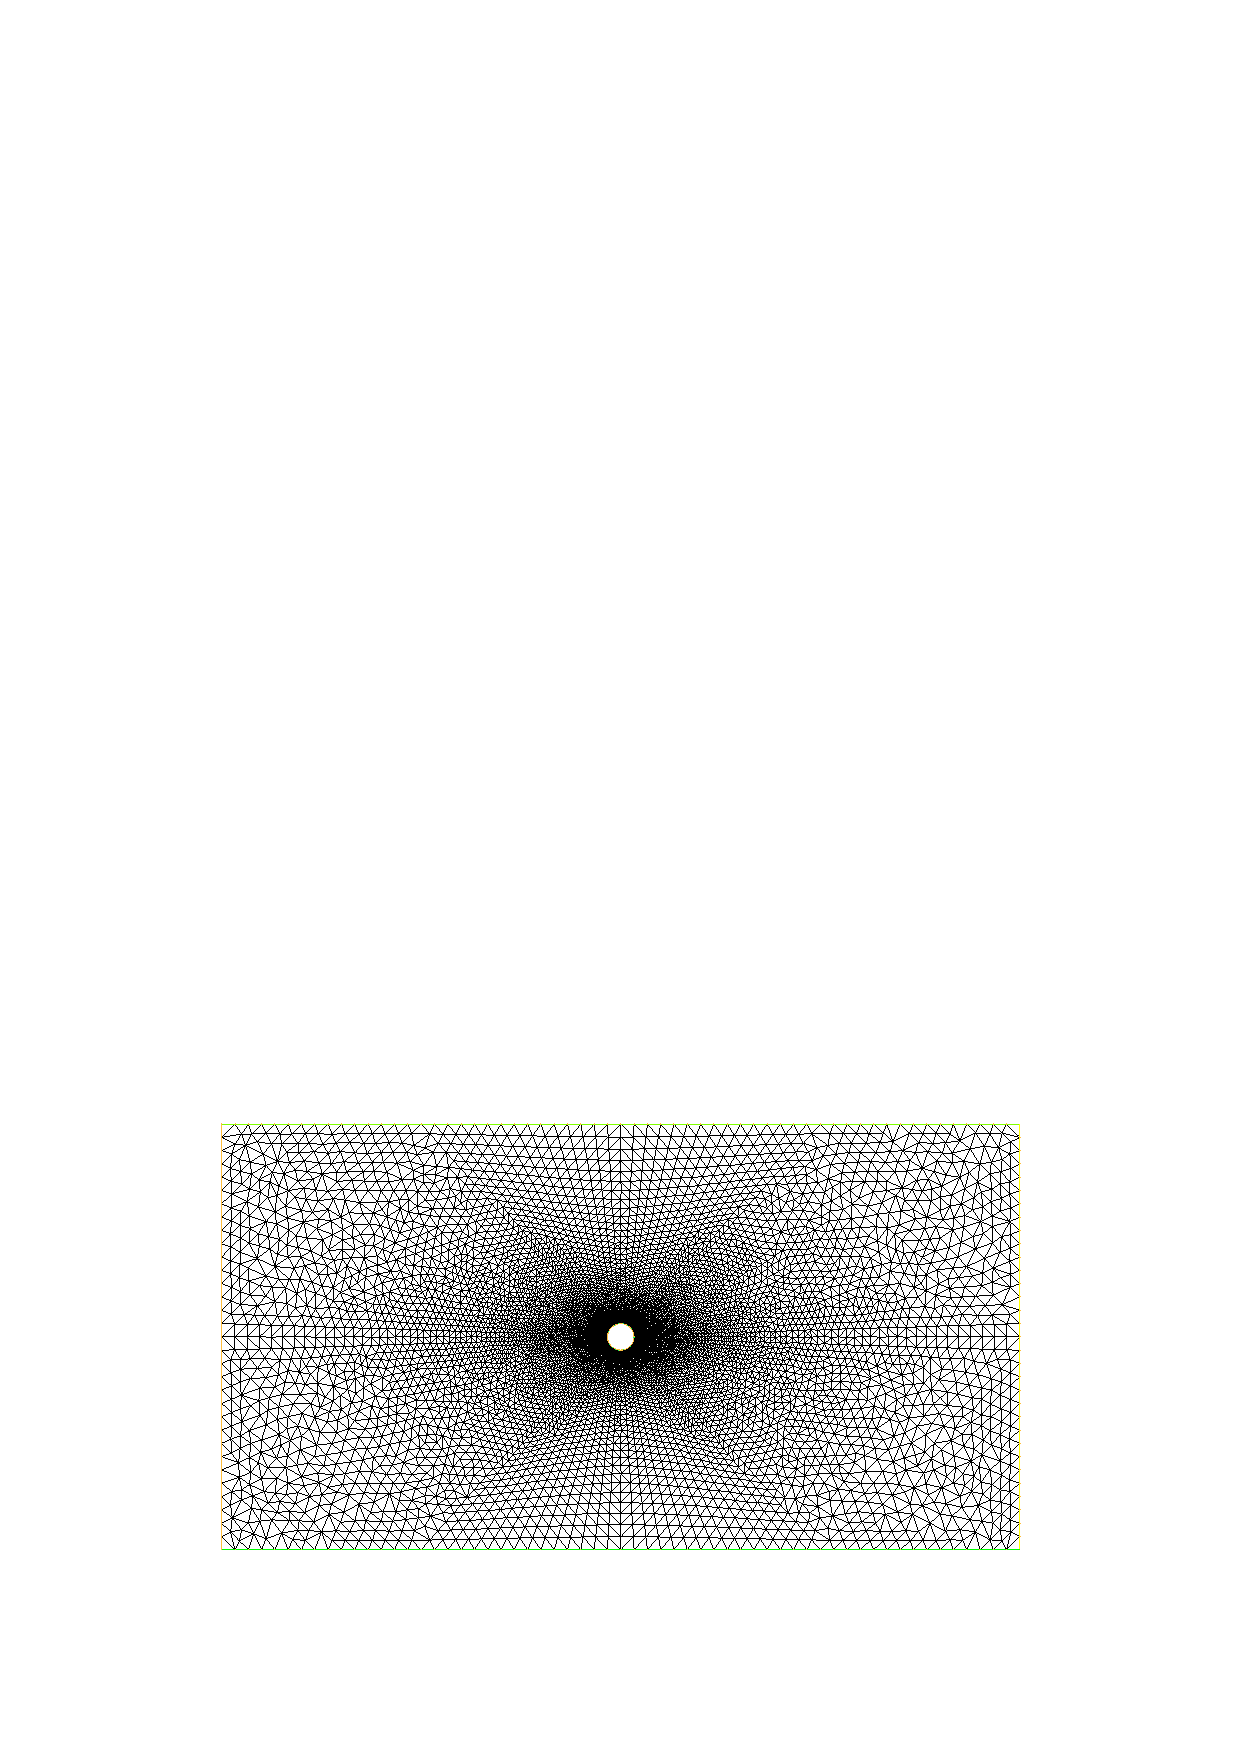
\includegraphics[width=\textwidth]{../n100/mesh.png}
    \caption{Unstructured mesh contructed in FreeFEM++ with 100 points on the cylinder body}
    \label{fig:mesh}
\end{figure}
\begin{figure}[H]
    \centering
    \includegraphics[width=\textwidth]{../n.png}
    \caption{Variation in the residual and pressure distribution over the surface with time for different number of points on the cylinder boundary}
    \label{fig:n}
\end{figure}

\begin{figure}[H]
    \centering
    \includegraphics[width=0.85\textwidth]{../n50/cyl.png}
    \caption{Velocity contour over the cylinder for 50 points on the cylinder surface.}
    \label{fig:cyl_n}
\end{figure}

\subsection{Variation of $\beta$}
$\beta$ is the user-defined parameter to control the artifical compressibility introduced in the equation. In general, the value of $\beta$ is choosen
less than one and a smaller value helps in faster convergence. Here, the domain size is kept unchanged with 100 points on the surface of
cylinder. The residual convergence is faster with increase in $\beta$. For $\beta = 10^{-5}$ the
$c_p$ plot is way off the potential solution, whereas for the case of $\beta = 10^{-7}$ and $\beta = 10^{-9}$, the $c_p$ plot coincides with the potential
flow solution. (\textbf{Figure \ref{fig:b}}). The solution converges for $\beta = 10^{-9}$ in 7 timesteps along with accuracy.

\begin{figure}[H]
    \centering
    \includegraphics[width=\textwidth]{../b.png}
    \caption{Variation in the residual and pressure distribution over the surface with time for different value of $\beta$.}
    \label{fig:b}
\end{figure}

\subsection{Variation with Domain}
The computational domain is enlarged from the original size of $20D\times12D$ to $30D\times16D$ and reduced to $10D\times8D$.
The mesh refinement  i.e. number of points on the surface is fixed as 100 whereas the $\beta$ is fixed as $10^{-9}$.
The solution rapidly diverges for the smaller domain of $10D\times8D$ whereas it converges for the other two domains quickly.
Spurious oscillations are also observed at the top and bottom points of the cylinder i.e. $\theta=90­°$ and $\theta=-90­°$ for
the smaller domain due to interference from the top and bottom walls. (\textbf{Figure \ref{fig:d}}).
\begin{figure}[H]
    \centering
    \includegraphics[width=\textwidth]{../d.png}
    \caption{Variation in the residual and pressure distribution over the surface with time for domain.}
    \label{fig:d}
\end{figure}

\section{Conclusion}
The computation converges quickly to an accurate steady-state solution for a large domain with mesh refinement near the body
and a small value of $\beta$. The domain should be large enough such that it doesn't interfere with the flow around the simulation
and far-field conditions are achieved.

\end{document} % This is the end of the document